\documentclass[border=3pt,tikz]{standalone}
\usepackage{amsmath} % for \text
\usepackage{etoolbox} % ifthen
\usepackage[outline]{contour} % glow around text
\usetikzlibrary{calc} % for adding up coordinates
\usetikzlibrary{decorations.markings,decorations.pathmorphing}
\usetikzlibrary{angles,quotes} % for pic (angle labels)
\usetikzlibrary{arrows.meta} % for arrow size
\usepackage{xfp} % higher precision (16 digits?)
\contourlength{1.1pt}

% COLORS
\colorlet{myred}{red!85!black}
\colorlet{mydarkred}{red!55!black}
\colorlet{mylightred}{red!85!black!12}
\colorlet{myfieldred}{mydarkred!5} % for S' background
\colorlet{myredhighlight}{myred!20} % highlights simultaneity in ladder paradox
\colorlet{myblue}{blue!80!black}
\colorlet{mydarkblue}{blue!50!black}
\colorlet{mylightblue}{blue!50!black!30}
\colorlet{mylightblue2}{myblue!10}
\colorlet{mygreen}{green!80!black}
\colorlet{mydarkgreen}{green!50!black}
\colorlet{mypurple}{blue!40!red!80!black}
\colorlet{mydarkpurple}{blue!40!red!50!black}
\colorlet{mypurple2}{blue!70!red!90!black}
\colorlet{mydarkpurple2}{blue!70!red!60!black}
\colorlet{myorange}{orange!40!yellow!95!black}
\colorlet{mydarkorange}{orange!40!yellow!85!black}
\colorlet{mybrown}{brown!20!orange!90!black}
\colorlet{mydarkbrown}{brown!20!orange!55!black}
\colorlet{mypurplehighlight}{mydarkpurple!20} % highlights simultaneity in ladder paradox

% STYLES
\tikzset{
	>=latex, % for LaTeX arrow head
	world line/.style={myblue!40,line width=0.2},
	world line t/.style={mypurple!50!myblue!40,line width=0.2},
	world line'/.style={mydarkred!40,line width=0.2},
	mysmallarr/.style={-{Latex[length=3,width=2]},thin},
	mydashed/.style={dash pattern=on 3 off 3},
	rod/.style={mydarkbrown,draw=mydarkbrown,double=mybrown,double distance=2pt,
		line width=0.2,line cap=round,shorten >=1pt,shorten <=1pt},
	%rod'/.style={rod,draw=mydarkbrown!80!red!85,double=mybrown!80!red!85},
	vector/.style={->,line width=1,line cap=round},
	vector'/.style={vector,shorten >=1.2},
	particle/.style={mygreen,line width=0.9},
	photon/.style={-{Latex[length=5,width=4]},myorange,line width=0.8,decorate,
		decoration={snake,amplitude=1.0,segment length=5,post length=5}}
}
\def\tick#1#2{\draw[thick] (#1) ++ (#2:0.06) --++ (#2-180:0.12)}
\def\tickp#1#2{\draw[thick,mydarkred] (#1) ++ (#2:0.06) --++ (#2-180:0.12)}
\def\Nsamples{100} % number samples in plot
\begin{document}
	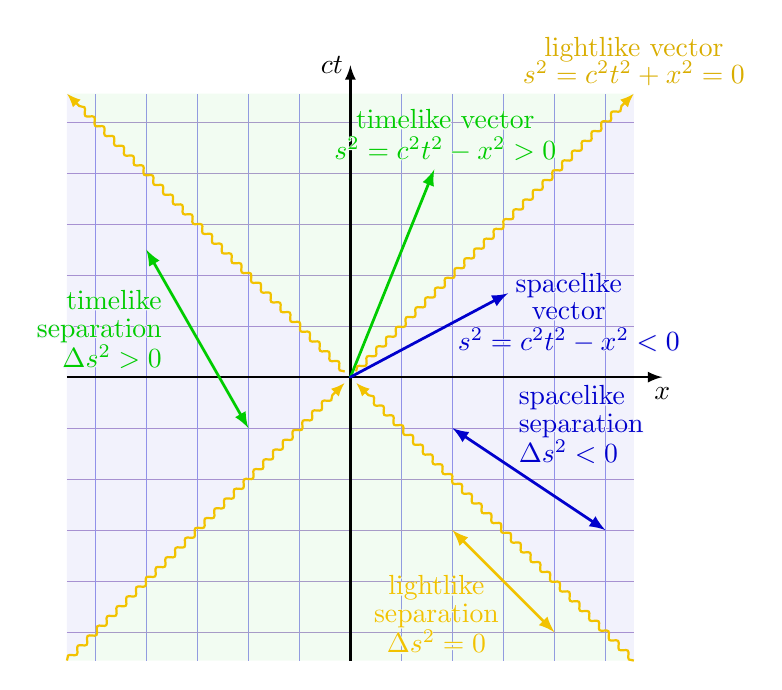
\begin{tikzpicture}[scale=1.8]
		\message{Vectors^^J}
		
		\def\xmax{2}
		\def\xmaxp{2.2} % maximum of rotated axis
		\def\Nlines{5} % number of world lines (at constant x/t)
		\pgfmathsetmacro\d{0.9*\xmax/\Nlines} % grid size
		\pgfmathsetmacro\ang{atan(1/3)} % angle between x and x' axes
		\coordinate (O) at (0,0);
		\coordinate (X) at (\xmax+0.2,0);
		\coordinate (T) at (0,\xmax+0.2);
		
		% WORLD LINE GRID
		\message{  Making world lines...^^J}
		\foreach \i [evaluate={\x=\i*\d;}] in {1,...,\Nlines}{
			\message{  Running i/N=\i/\Nlines, x=\x...^^J}
			\draw[world line]   (-\x,-\xmax) -- (-\x,\xmax);
			\draw[world line]   ( \x,-\xmax) -- ( \x,\xmax);
			\draw[world line t] (-\xmax,-\x) -- (\xmax,-\x);
			\draw[world line t] (-\xmax, \x) -- (\xmax, \x);
		}
		
		% FILLS
		\fill[myblue,opacity=0.05] % SPACELIKE
		(\xmax,\xmax) -- (-\xmax,-\xmax) -- (-\xmax,\xmax) -- (\xmax,-\xmax) -- cycle;
		\fill[mygreen,opacity=0.05] % TIMELIKE
		(\xmax,\xmax) -- (-\xmax,\xmax) -- (\xmax,-\xmax) -- (-\xmax,-\xmax) -- cycle;
		
		% AXES
		\draw[->,thick] (0,-\xmax) -- (T) node[left=-1] {$ct$};
		\draw[->,thick] (-\xmax,0) -- (X) node[below=0] {$x$};
		
		% VECTORS
		\draw[vector,mygreen] (O) --++ (68:0.79*\xmax)
		node[right=4,above=-1,align=center]
		{\contour{mygreen!5}{timelike vector}\\[-1]
			\contour{mygreen!5}{$s^2=c^2t^2-x^2>0$}};
		\draw[vector,myblue] (O) --++ (28:0.63*\xmax)
		node[below=7,right=-22,align=center]
		{\contour{myblue!5}{spacelike}\\[-2]
			\contour{myblue!5}{vector}\\[-1]
			\contour{myblue!5}{$s^2=c^2t^2-x^2<0$}};
		\draw[vector,mygreen,<->] (-2*\d,-\d) --++ (-2*\d,3.5*\d)
		node[pos=0.8,below left=-2,align=right]
		{\contour{myblue!5}{timelike}\\[-2]
			\contour{myblue!5}{separation}\\[-1]
			\contour{myblue!5}{$\Delta s^2>0$}};
		\draw[vector,myblue,<->] (2*\d,-\d) --++ (3*\d,-2*\d)
		node[pos=0.4,above right=-2,align=left]
		{\contour{myblue!5}{spacelike}\\[-2]
			\contour{myblue!5}{separation}\\[-1]
			\contour{myblue!5}{$\Delta s^2<0$}};
		\draw[vector,myorange,<->] (2*\d,-3*\d) --++ (2*\d,-2*\d)
		node[pos=0.45,below left=-4,align=center]
		{\contour{mygreen!5}{lightlike}\\[-2]
			\contour{mygreen!5}{separation}\\[-1]
			\contour{mygreen!5}{$\Delta s^2 = 0$}};
		
		% PHOTON
		\draw[photon] ( \xmax,-\xmax) -- ( 0.02*\xmax,-0.02*\xmax);
		\draw[photon] (-\xmax,-\xmax) -- (-0.02*\xmax,-0.02*\xmax);
		\draw[photon] ( 0.02*\xmax,0.02*\xmax) -- ( \xmax,\xmax)
		node[mydarkorange,above=-1,align=center] {lightlike vector\\[-2]$s^2=c^2t^2+x^2=0$};
		\draw[photon] (-0.02*\xmax,0.02*\xmax) -- (-\xmax,\xmax);
		
	\end{tikzpicture}
\end{document}
